\documentclass[11pt,a5paper,fleqn,leqno]{book}
\usepackage[utf8x]{inputenc}
\usepackage{ucs}
\usepackage{amsmath}
\usepackage{amsfonts}
\usepackage{icomma}
\usepackage{amssymb}
\usepackage{graphicx}
\usepackage{enumerate}
\usepackage[top=2.5cm, bottom=2.5cm, left=1.25cm, right=1.25cm]{geometry}
\usepackage{ifpdf}
\ifpdf
  \DeclareGraphicsRule{*}{mps}{*}{}
\fi
\usepackage[danish]{babel}
\usepackage[pdftex,
	pdfauthor={Frank Bille},
	pdftitle={Formelsamling},
	bookmarks=true,
	colorlinks,
	linkcolor=black
]
{hyperref}
\author{Frank Bille}
\title{Formelsamling}

\begin{document}

\setlength{\parindent}{0cm}

\frontmatter

\thispagestyle{empty}
\setlength{\arrayrulewidth}{0.1cm}
\null
\begin{flushright}
  \begin{tabular}{r|}
    \rule{0pt}{3ex} \\
    \rule{0pt}{3ex} \\
    \Huge \textsf{\textbf{Formelsamling}}
    \rule{0pt}{4ex} \\
    \large \textsf{Frank Bille Jensen}
    \rule{0pt}{3ex} \\
    \rule{0pt}{3ex} \\
    \rule{0pt}{3ex} \\
    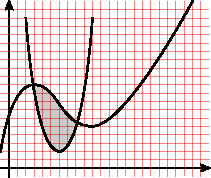
\includegraphics[width=9.5cm]{cover.pdf} \\
    \rule{0pt}{3ex} \\
    \rule{0pt}{3ex} \\
    \rule{0pt}{3ex} \\
  \end{tabular}
\end{flushright}
\cleardoublepage
\setlength{\arrayrulewidth}{0.4pt}

\tableofcontents

\mainmatter

\pagestyle{headings}

\chapter{Formler og regneregler}

\newpage

\section{Areal og omkreds}

\subsection{Rektangel}

\includegraphics{graph.6}
\\
\\
Højde $h$ \\
Grundlinje $g$ \\
Areal $A$
\begin{equation} \label{eq:areal_rektangle}
A = h \cdot g
\end{equation}

\subsection{Parallelogram}

\includegraphics{graph.7}
\\
\\
Højde $h$ \\
Grundlinje $g$ \\
Areal $A$
\begin{equation}
A = h \cdot g
\end{equation}

\subsection{Kvadrat}

\includegraphics{graph.5}
\\
\\
Sidelængde $a$ \\
Areal $A$
\begin{equation}
A = a \cdot a = a^2
\end{equation}

\subsection{Trekant}

\includegraphics{graph.4}
\\
\\
Højde $h$ \\
Grundlinje $g$ \\
Areal $A$ \\
Omkreds $O$
\begin{equation} \label{eq:areal_trekant}
A = \frac{1}{2} \cdot h \cdot g
\end{equation}
\begin{equation}
O = |AB| + |BC| + |CA|
\end{equation}

\subsection{Trapez}

\includegraphics{graph.8}
\\
\\
Højde $h$ \\
Parallelle sider $a$ og $b$ \\
Areal $A$
\begin{equation}
A = \frac{1}{2} \cdot h \cdot (a + b)
\end{equation}

\subsection{Cirkel}

\includegraphics{graph.9}
\\
\\
Radius $r$ \\
Areal $A$ \\
Omkreds $O$
\begin{equation} \label{eq:areal_cirkel}
A = \pi \cdot r^2
\end{equation}

\begin{equation} \label{eq:omkreds_cirkel}
O = 2 \cdot \pi \cdot r
\end{equation}

\section{Brøker}

\begin{equation} \label{eq:taeller_naevner_det_samme}
\frac{a}{a} = 1
\end{equation}

\begin{equation} \label{eq:konstant_gange_med_broek}
a \cdot \frac{b}{c} = \frac{a \cdot b}{c} = \frac{a}{c} \cdot b
\end{equation}

\begin{equation} \label{eq:broeker_med_ens_naevnere_plusminus}
\frac{a}{b} \pm \frac{c}{b} = \frac{a \pm c}{b}
\end{equation}

\begin{equation} \label{eq:broeker_med_forskellige_naevnere_plusminus}
\frac{a}{b} \pm \frac{c}{d} = \frac{a \cdot d \pm c \cdot b}{b \cdot d}
\end{equation}

\begin{equation} \label{eq:broeker_ganget_sammen}
\frac{a}{b} \cdot \frac{c}{d} = \frac{a \cdot c}{b \cdot d}
\end{equation}

\begin{equation} \label{eq:forlaenge_en_broek}
\frac{a}{b} = 1 \cdot \frac{a}{b} = \frac{c}{c} \cdot \frac{a}{b} = \frac{c \cdot a}{c \cdot b}
\end{equation}

\begin{equation} \label{eq:broeker_divideret}
\frac{\frac{a}{b}}{\frac{c}{d}} = \frac{a}{b} \cdot \frac{d}{c}
\end{equation}

\newpage

\section{Ligninger}

Generelt for ligninger gælder det at de operationer man foretager på den ene side af lighedstegnet også skal udføres på den anden side af lighedstegnet.
\\
\\
Isolere $x$ ved at trække $a$ fra på begge sider af lighedstegnet
\begin{equation} \label{eq:ligning_minus}
x + a = b \Leftrightarrow x + a - a = b - a \Leftrightarrow x = b - a
\end{equation}

Isolere $x$ ved at ligge $a$ til på begge sider af lighedstegnet
\begin{equation} \label{eq:ligning_plus}
x - a = b \Leftrightarrow x - a + a = b + a \Leftrightarrow x = b + a
\end{equation}

Isolere $x$ ved at dividere med $a$ på begge sider af lighedstegnet
\begin{equation} \label{eq:ligning_dividere}
a \cdot x = b \Leftrightarrow \frac{a \cdot x}{a} = \frac{b}{a} \Leftrightarrow \frac{a}{a} \cdot x = \frac{b}{a} \Leftrightarrow x = \frac{b}{a}
\end{equation}

Isolere $x$ ved at gange med $a$ på begge sider af lighedstegnet
\begin{equation} \label{eq:ligning_gange}
\frac{x}{a} = b \Leftrightarrow \frac{x}{a} \cdot a = b \cdot a \Leftrightarrow x \cdot \frac{a}{a} = b \cdot a \Leftrightarrow x = b \cdot a
\end{equation}

Isolere $x$ ved at tage kvadratrodden på begge sider af lighedstegnet
\begin{equation} \label{eq:ligning_kvadratrod}
x^2 = b \Leftrightarrow \sqrt{x^2} = \sqrt{b} \Leftrightarrow x = \sqrt{b}
\end{equation}

\newpage

\section{Procentregning}

\begin{eqnarray} \label{eq:procent}
\% & = & \frac{1}{100} \\
a\% & = & a \cdot \frac{1}{100} = \frac{a}{100} \nonumber
\end{eqnarray}
\\
\\
Beregne procent $a$ af $b$
\begin{equation} \label{eq:procent_beregne}
a\% \; \text{af} \; b = \frac{a}{100} \cdot b = \frac{a \cdot b}{100} = a \cdot \frac{b}{100}
\end{equation}
\\
\\
Finde $a$'s forhold til $b$ udtrykt som procent
\begin{equation} \label{eq:procent_finde}
\frac{a}{b} \cdot 100\% 
\end{equation}
\\
\\
Kapitalfremskrivning \\
Startkapital $K_0$ \\
Rentefod $r$ \\
Kapital $K$ efter $n$ terminer
\begin{equation} \label{eq:procent_kapital}
K = K_{0} \cdot \left(1+r\right)^{n}
\end{equation}
\\
\\
Gennemsnitlig procentvis ændring $r$
\begin{equation} \label{eq:procent_gennemsnit_aendring}
1+r = \sqrt[n]{\left(1+r_{1}\right) \cdot \left(1+r_{2}\right) \cdot ... \cdot \left(1+r_{n}\right)}
\end{equation} 

\newpage

\section{Potensregneregler}

\begin{equation} \label{eq:potens}
a^r = 1 \cdot a_1 \cdot a_2 \cdot ... \cdot a_r
\end{equation}

\begin{equation} \label{eq:potens_gange}
a^r \cdot a^s = a^{r+s}
\end{equation}

\begin{equation} \label{eq:potens_dividere}
\dfrac{a^r}{a^s} = a^{r-s}
\end{equation}

\begin{equation} \label{eq:potens_potens}
\left(a^r\right)^s = a^{r \cdot s}
\end{equation}

\begin{equation} \label{eq:potens_faktorer}
\left(a \cdot b\right)^{r} = a^{r} \cdot b^{r}
\end{equation}

\begin{equation} \label{eq:potens_divisor}
\left(\dfrac{a}{b}\right)^{r} = \dfrac{a^{r}}{b^{r}}
\end{equation}

\begin{equation} \label{eq:potens_nulte}
a^{0} = 1
\end{equation}

\begin{equation} \label{eq:potens_minuste}
a^{-r} = \dfrac{1}{a^{r}}
\end{equation}

\begin{equation} \label{eq:potens_kvadratrod}
\sqrt[r]{a} = a^{\frac{1}{r}}
\end{equation}

\begin{equation} \label{eq:potens_kvadratrod_potens}
\sqrt[s]{a^{r}} = a^{\frac{r}{s}}
\end{equation}

\vfill

\section{Proportionalitet}

Proportionale størrelse $x$ og $y$
\begin{eqnarray}
y & =&  k \cdot x \\
\frac{y}{x} & = & k \nonumber
\end{eqnarray}
\\
\\
Omvendt proportionale størrelser $x$ og $y$
\begin{eqnarray}
y & = & c \cdot \frac{1}{x} \\
x \cdot y & = & c \nonumber
\end{eqnarray}

\section{Cirkel}

\includegraphics{graph.12}
\\
\\
Ligning for cirkel med centrum i $C(a,b)$ og radius $r$
\begin{equation}
(x-a)^2 + (y-b)^2 = r^2
\end{equation}

\newpage

\section{Koordinatsystem i planen}

\includegraphics{graph.1}

Afstanden $|AB|$ mellem to punkter $A(x_1,y_1)$ og $B(x_2,y_2)$
\begin{equation}
|AB| = \sqrt{(x_2-x_1)^2 + (y_2-y_1)^2}
\end{equation}
\\
\\
\includegraphics{graph.2}

Midtpunkt $M$ af linjestykke $AB$
\begin{equation}
M\left(\frac{x_1+x_2}{2},\frac{y_1+y_2}{2}\right)
\end{equation}

\vfill

\section{Linje}

\includegraphics{graph.3}
\\
\\
Ligninger for linjen $l$
\begin{eqnarray} \label{eq:linje_ligning}
y     & = & ax+b \\
y-y_1 & = & a(x-x_1) \nonumber
\end{eqnarray}
\\
\\
Hældningskoefficent (stigningstal) $a$ for linjen $l$
\begin{equation} \label{eq:linje_haeldning}
a = \frac{y_2 - y_1}{x_2 - x_1}
\end{equation}
\begin{equation}
a = \tan v
\end{equation}

\newpage

\includegraphics{graph.10}
\\
\\
Ortogonale linjer $l$ og $m$
\begin{equation}
l \perp m \Leftrightarrow a \cdot c = -1
\end{equation}
\\
\\
\includegraphics{graph.11}
\\
\\
Afstand $\text{dist}(P,l)$ fra punktet $P(x_1,y_1)$ til linjen $l$ med ligningen $y = ax+b$
\begin{equation}
\text{dist}(P,l) = \frac{|ax_1 + b - y_1|}{\sqrt{a^2 + 1}}
\end{equation}

\vfill

\section{Parabel}

\includegraphics{graph.13}
\\
\\
Ligning for parabel med symmetriakse parallel med andenaksen
\begin{equation}
y = ax^2 + bx +c
\end{equation}
\\
\\
Toppunkt $T$
\begin{equation} \label{eq:parabel_toppunkt}
T\left(\frac{-b}{2a}, \frac{-d}{4a}\right), \quad \text{hvor} \quad d = b^2 - 4ac
\end{equation}
\\
Skæringspunkter $S_1$ og $S_2$ med førsteaksen
\begin{equation} \label{eq:parabel_roedder}
S_1\left(\frac{-b - \sqrt{d}}{2a}, 0\right), \quad S_2\left(\frac{-b + \sqrt{d}}{2a}, 0\right)
\end{equation}

\newpage

\section{Trekant}

\subsection{Ensvinklede trekanter}

\includegraphics{graph.14}

\begin{equation}
\frac{a_1}{a} = \frac{b_1}{b} = \frac{c_1}{c} = k
\end{equation}

\begin{eqnarray}
a_1 & = & k \cdot a \\
b_1 & = & k \cdot b \nonumber \\
c_1 & = & k \cdot c \nonumber
\end{eqnarray}

\vfill

\subsection{Retvinklet trekant}

\includegraphics{graph.15}
\\
\\
Pythagoras' læresætning, hvor $a$ og $b$ er katetere og $c$ er hypotenusen.
\begin{equation} \label{eq:trekant_pythagoras}
a^2 + b^2 = c^2
\end{equation}

\begin{equation}
\sin A = \frac{a}{c}
\end{equation}

\begin{equation}
\cos A = \frac{b}{c}
\end{equation}

\begin{equation}
\tan A = \frac{a}{b}
\end{equation}

\vfill

\subsection{Vilkårlig trekant}

\includegraphics{graph.16}
\\
\\
Cosinusrelation
\begin{equation}
c^2 = a^2 + b^2 - 2ab\cos C
\end{equation}
\\
\\
Sinusrelation
\begin{equation}
\frac{a}{\sin A} = \frac{b}{\sin B} = \frac{c}{\sin C}
\end{equation}
\\
\\
Trekantens areal $T$ \\
Højden på $c$ = $h_c$
\begin{eqnarray}
T & = & \frac{1}{2}h_c a \\
& = & \frac{1}{2}ab\sin C \nonumber
\end{eqnarray}

\newpage

\section{Polynomier}

\subsection{Førstegradspolynomium}

\includegraphics{graph.17}
\\
\\
Førstegradspolynomium, lineær funktion $f$
\begin{equation}
f(x) = ax+b
\end{equation}

\newpage

\subsection{Andengradspolynomium}

\includegraphics{graph.18}
\\
\\
Andengradspolynomium $p$ med rødder $x_1$ og $x_2$
\begin{eqnarray}
p(x) & = & ax^2 + bx + c \\
 & = & a(x-x_1)(x-x_2) \nonumber
\end{eqnarray}
\\
\\
Rødder i andengradspolynomium $p$
\begin{equation}
x_1 = \frac{-b - \sqrt{d}}{2a}, \quad \frac{-b + \sqrt{d}}{2a}, \quad \text{hvor} \quad d = b^2 - 4ac
\end{equation}
\\
\\
Polynomium $p$ af grad $n$
\begin{equation}
p(x) = a_nx^n + a_{n-1}x^{n-1} + \dots + a_1x + a_0
\end{equation}

\vfill

\section{Logaritmefunktioner}

\includegraphics{graph.21}
\\
\\
Grafer for $y = \log x$ og $y = 10^x$
\begin{equation}
y = \log x \Leftrightarrow x = 10^y
\end{equation}
\\
\\
Logaritmefunktionen $\log$ med grundtal 10
\begin{equation}
\log 10 = 1
\end{equation}
\begin{equation}
\log(a \cdot b) = \log a + \log b
\end{equation}
\begin{equation}
\log\left(\frac{a}{b}\right) = \log a - \log b
\end{equation}
\begin{equation}
\log(a^r) = r \cdot \log a
\end{equation}

\newpage

\includegraphics{graph.22}
\\
\\
Grafer for $y = \ln x$ og $y = e^x$
\begin{equation}
y = \ln x \Leftrightarrow x = e^y
\end{equation}
\\
\\
Den naturlige logaritmefunktion $\ln$ med grundtal $e$
\begin{equation}
\ln e = 1
\end{equation}
\begin{equation}
\ln (a \cdot b) = \ln a + \ln b
\end{equation}
\begin{equation}
\ln\left(\frac{a}{b}\right) = \ln a - \ln b
\end{equation}
\begin{equation}
\ln(a^r) = r \cdot \ln a
\end{equation}

\newpage

\section{Eksponentialfunktioner}

\includegraphics{graph.23}
\\
\\
Grafer for $y = a^x$ og $y = b \cdot a^x$ i enkeltlogaritmisk koordinatsystem.
\\
\\
Eksponentialfunktion
\begin{equation}
f(x) = a^x
\end{equation}
\\
\\
Funktion, der er proportional med en eksponentialfunktion
\begin{equation}
f(x) = b \cdot a^x
\end{equation}
\\
\\
\includegraphics{graph.24}
\\
\\
Bestemmelse af fremskivningsfaktor $a$
\begin{equation}
a = \sqrt[x_2-x_1]{\frac{y_2}{y_1}}
\end{equation}
\\
\\
En eksponentielt voksende funktion $f$ med fremskrivningsfaktor $a$, hvor $a > 1$, dvs. med vækstrate $r$, hvor $r > 0$
\begin{eqnarray}
f(x) & = & b \cdot a^x \\
 & = & b \cdot (1+r)^x \nonumber \\
 & = & b \cdot e^{kx}, \quad \text{hvor} \quad k = \ln a \nonumber
\end{eqnarray}

\newpage

\includegraphics{graph.25}
\\
\\
Fordoblingskonstant $T_2$
\begin{equation}
T_2 = x_2 - x_1
\end{equation}

\begin{equation}
T_2 = \frac{\log 2}{\log a} = \frac{\ln 2}{\ln a} = \frac{\ln 2}{k}
\end{equation}

\begin{equation}
b \cdot a^x = b \cdot e^{kx} = b \cdot 2^{\frac{x}{T_2}}
\end{equation}
\\
\\
En eksponentielt aftagende funktion $f$ med fremskrivningsfaktor $a$, hvor $0 < a < 1$, dvs. med vækstrate $-r$, hvor $r > 0$
\begin{eqnarray}
f(x) & = & b \cdot a^x \\
 & = & b \cdot (1-r)^x \nonumber \\
 & = & b \cdot e^{-kx}, \quad \text{hvor} \quad k = -\ln a \nonumber
\end{eqnarray}
\\
\\
\includegraphics{graph.26}
\\
\\
Halveringskonstant $T_{\frac{1}{2}}$
\begin{equation}
T_{\frac{1}{2}} = x_2 - x_1
\end{equation}

\begin{equation}
T_{\frac{1}{2}} = \frac{\log\left(\frac{1}{2}\right)}{\log a} = \frac{\ln\left(\frac{1}{2}\right)}{\ln a} = \frac{\ln\left(\frac{1}{2}\right)}{-k}
\end{equation}

\begin{equation}
b \cdot a^x = b \cdot e^{-kx} = b \cdot \left(\frac{1}{2}\right)^{\frac{x}{T_{\frac{1}{2}}}}
\end{equation}

\newpage

\section{Potensfunktioner}

\includegraphics{graph.27}
\\
\\
Grafer for $y = x^a$ og $y = b \cdot x^a$ i dobbeltlogaritmisk koordinatsystem
\\
\\
Potensfunktion
\begin{equation}
f(x) = x^a = e^{a\ln x}
\end{equation}
\begin{equation}
y = x^a \Leftrightarrow x = \sqrt[a]{y}
\end{equation}
\\
\\
Funktion, der er proportional med en potensfunktion
\begin{equation}
f(x) = b \cdot x^a
\end{equation}

\newpage

\includegraphics{graph.28}
\\
\\
Bestemmelse af eksponenten $a$
\begin{equation}
a = \frac{\log y_2 - \log y_1}{\log x_2 - \log x_1} = \frac{\ln y_2 - \ln y_1}{\ln x_2 - \ln x_1}
\end{equation}
\\
\\
Funktion $f$ defineres som $f(x) = b \cdot x^a$. $f(x)$ fremskrives med faktor $q^a$, når $x$ fremskrives med faktor $q$
\begin{equation}
f(q \cdot x) = q^a \cdot f(x)
\end{equation}

\vfill

\section{Trigonometriske funktioner}

\includegraphics{graph.19}
\\
\\
Aflæsning af $\cos x$ og $\sin x$
\begin{equation}
(\cos x)^2 + (\sin x)^2 = 1
\end{equation}
\begin{eqnarray}
\cos(x + 2\pi) & = & \cos x \\
\sin(x + 2\pi) & = & \sin x \nonumber
\end{eqnarray}
\begin{eqnarray}
\cos(-x) & = & \cos x \\
\sin(-x) & = & - \sin x \nonumber
\end{eqnarray}
\begin{eqnarray}
\cos(\pi - x) & = & - \cos x \\
\sin(\pi - x) & = & \sin x \nonumber
\end{eqnarray}
\begin{eqnarray}
\cos\left(\frac{\pi}{2}-x\right) & = & \sin x \\
\sin\left(\frac{\pi}{2}-x\right) & = & \cos x \nonumber
\end{eqnarray}

\includegraphics{graph.20}
\\
\\
Aflæsning af $\tan x$
\begin{equation}
\tan x = \frac{\sin x}{\cos x}
\end{equation}
\begin{equation}
\tan(-x) = -\tan x
\end{equation}
\begin{equation}
\tan(x+\pi) = \tan x
\end{equation}

\newpage

\section{Differentialregning}

\includegraphics{graph.29}
\\
\\
Ligning for tangent $t$ i punktet $A(x_0,f(x_0))$
\begin{equation} \label{eq:diff_tangent_t}
y = f(x_0) + f'(x_0)(x-x_0)
\end{equation}
\\
Approximerede førstegradspolynomium $p$ for $f$ i tallet $x_0$
\begin{equation} \label{eq:diff_tangent_p}
p(x) = f(x_0) + f'(x_0)(x-x_0)
\end{equation}
\\
Regneregler for differentiation
\begin{eqnarray}
\left(f \pm g\right)'(x)     & = & f'(x) \pm g'(x) \\
\left(f \cdot g\right)'(x)   & = & f'(x) \cdot g(x) + f(x) \cdot g'(x) \\
\left(k \cdot f\right)'(x)   & = & k \cdot f'(x) \\
\left(\frac{f}{g}\right)'(x) & = & \dfrac{f'(x) \cdot g(x) - f(x) \cdot g'(x)}{\left(g(x)\right)^2} \\
\left(f \circ g\right)'(x)   & = & \left(f\left(g(x)\right)\right)' = f'\left(g(x)\right) \cdot g'(x)
\end{eqnarray}

\vfill

\section{Regneregler for integration}

I dette afsnit betegner $F$ en stamfunktion til $f$

\paragraph{Ubestemt integral}

\begin{equation}
\int f(x)\, \mathrm{d}x = F(x) + c
\end{equation}

\begin{equation}
\int \left(f(x) \pm g(x)\right)\, \mathrm{d}x = \int f(x)\, \mathrm{d}x \pm \int g(x)\, \mathrm{d}x
\end{equation}

\begin{equation}
\int k \cdot f(x)\, \mathrm{d}x = k \cdot \int f(x)\, \mathrm{d}x
\end{equation}

\begin{equation}
\int f(x) \cdot g(x)\, \mathrm{d}x = F(x) \cdot g(x) -  \int F(x) \cdot g'(x)\, \mathrm{d}x
\end{equation}

\begin{equation}
\int f(g(x)) \cdot g'(x)\, \mathrm{d}x = \int f(t)\, \mathrm{d}t \quad \mbox{hvor} \quad t = g(x)
\end{equation}

\paragraph{Bestemt integral}

\begin{equation}
\int_a^b f(x)\, \mathrm{d}x = \left[F(x)\right]_a^b = F(b) - F(a)
\end{equation}

\begin{equation}
\int_a^b f(x)\, \mathrm{d}x = \int_a^c f(x)\, \mathrm{d}x + \int_b^c f(x)\, \mathrm{d}x
\end{equation}

\begin{equation}
\int_a^b \left(f(x) \pm g(x)\right)\, \mathrm{d}x = \int_a^b f(x)\, \mathrm{d}x \pm \int_a^b g(x)\, \mathrm{d}x
\end{equation}

\begin{equation}
\int_a^b k \cdot f(x)\, \mathrm{d}x = k \cdot \int_a^b f(x)\, \mathrm{d}x
\end{equation}

\begin{equation}
\int_a^b k \cdot f(x)\, \mathrm{d}x = k \cdot \int_a^b f(x)\, \mathrm{d}x
\end{equation}

\begin{equation}
\int_a^b f(x) \cdot g(x)\, \mathrm{d}x = \left[F(x) \cdot g(x) \right]_a^b - \int_a^b F(x) \cdot g'(x)\, \mathrm{d}x
\end{equation}

\begin{eqnarray}
\int_a^b f(g(x)) \cdot g'(x)\, \mathrm{d}x & = & \int_{g(a)}^{g(b)} f(t)\, \mathrm{d}t  \quad \mbox{hvor} \quad t = g(x) \\
 & = & F(g(b)) - F(g(a)) \nonumber
\end{eqnarray}

\chapter{Opgaver} \label{ch:Opgaver}

Opgaverne kan løses ved hjælpe af formlerne i denne formelsamling. Du kan finde løsningerne i kapitel \ref{ch:Loesninger} på side \pageref{ch:Loesninger}.

De fleste opgaver er lavet så der ikke behøves lommeregner.

\newpage

\section{Areal og omkreds}

\begin{enumerate}
\item \label{op:areal_1} Beregn arealet af et \textit{rektangel} når højden er 4cm og grundlinjen er 7cm.
\item \label{op:areal_2} Beregn arealet af en trekant med højden 2cm og grundlinjen 7cm.
\item \label{op:areal_3} En cirkel har en diameter på 8cm. Hvor stor er omkredsen på denne cirkel?
\end{enumerate}

\section{Brøker}

Reducér følgende brøker

\begin{enumerate}
\item \label{op:broek_1} $4 \cdot \frac{5}{4}$
\item \label{op:broek_2} $\frac{7}{2} - \frac{8}{6}$
\item \label{op:broek_3} $\frac{\frac{3}{4}}{\frac{9}{4}}$
\end{enumerate}

\section{Ligninger}

Isoler $a$ i følgende ligninger

\begin{enumerate}
\item \label{op:ligning_1} $a-3=7$
\item \label{op:ligning_2} $2a+10=-16$
\item \label{op:ligning_3} $a+2a-3 = 5a -5$
\end{enumerate}

\section{Procentregning}

\begin{enumerate}
\item \label{op:procent_1} En person tjener 28000kr om måneden, men skal betale 39\% i skat. Hvor meget får vedkommende udbetalt hver måned efter at skatten er trukket fra?
\item \label{op:procent_2} 110m hækkeløb er en diciplin ved de Olympiske Lege. Løberne løber en distance på 110 meter hvor der er en række forhindringer som de skal hoppe over. Afstanden fra startlinjen til den første hæk er 13,72m. Hvor mange procent har løberne gennemført når de når til den første hæk?
\end{enumerate}

\section{Potensregneregler}

Reducér følgende potenser

\begin{enumerate}
\item \label{op:potens_1} $1 \cdot 2 \cdot 2 \cdot 2 \cdot 2 \cdot 2 \cdot 2 \cdot 2$
\item \label{op:potens_2} $3^3 \cdot 3^4$
\item \label{op:potens_3} $2^0$
\item \label{op:potens_4} $\sqrt{3} \cdot 3^2$
\item \label{op:potens_5} $\sqrt{5}^2$
\item \label{op:potens_6} $\sqrt{5^2}$
\end{enumerate}

\section{Linje}

\begin{enumerate}
\item \label{op:linje_1} Den rette linje $l$ går i gennem to punkter $A(1,3)$ og $B(2,5)$. Find ligningen for linjen $l$
\end{enumerate}

\section{Parabel}

\begin{enumerate}
\item \label{op:parabel_1} Find rødderne og toppunktet i andengradsligningen $y = 2x^2 - 5x + 2$
\end{enumerate}

\section{Trekant}

\begin{enumerate}
\item \label{op:trekant_1}
Beregn længden af linjestykket $c$. \\
\includegraphics{graph.30}
\item \label{op:trekant_2}
Beregn længden af linjestykket $b$. \\
\includegraphics{graph.31}
\end{enumerate}

\section{Differentialregning}

\begin{enumerate}
\item \label{op:diff_1} Funktionen $f$ er defineret som $f(x) = \frac{1}{2}x^2 - 3x + 2$. Bestem foreskriften for tangenten $t$ i punktet $A(2,-2)$.
\end{enumerate}

\chapter{Løsninger} \label{ch:Loesninger}

Alle løsningerne er så detaljerede som muligt og vil for det meste indeholde referencer til de formler der er benyttet.

\newpage

\section{Areal og omkreds}

\ref{op:areal_1}. Benytter \eqref{eq:areal_rektangle}
\begin{displaymath}\begin{array}{l}
h = 4\text{cm}\\
g = 7\text{cm}\\
A = h \cdot g = 4\text{cm} \cdot 7\text{cm} = \underline{\underline{28\text{cm}^2}}
\end{array}\end{displaymath}

\ref{op:areal_2}. Benytter \eqref{eq:areal_trekant}
\begin{displaymath}\begin{array}{l}
h = 2\text{cm}\\
g = 7\text{cm}\\
A = \frac{1}{2} \cdot h \cdot g = \frac{1}{2} \cdot 2\text{cm} \cdot 7\text{cm} = \underline{\underline{7\text{cm}^2}}
\end{array}\end{displaymath}

\ref{op:areal_3}. Diameteren $d$ på en cirkel er 2 gange radius. Det vil sige at radius er
\[r = \frac{d}{2} = \frac{8\text{cm}}{2} = \underline{4\text{cm}}\]
Ved at benytte \eqref{eq:omkreds_cirkel}, kan vi så beregne omkredsen.
\[O = 2 \cdot \pi \cdot r = 2 \cdot \pi \cdot 4\text{cm} \simeq \underline{\underline{25,13\text{cm}}}\]

\section{Brøker}

\ref{op:broek_1}. Benytter: \eqref{eq:konstant_gange_med_broek}
\[4 \cdot \frac{5}{4} = \frac{4 \cdot 5}{4} = \frac{4}{4} \cdot 5 = \underline{\underline{5}}\]

\ref{op:broek_2}. Benytter: \eqref{eq:broeker_med_forskellige_naevnere_plusminus}, \eqref{eq:broeker_ganget_sammen} og \eqref{eq:forlaenge_en_broek}
\[\frac{7}{2} - \frac{8}{6} = \frac{7 \cdot 6 - 8 \cdot 2}{2 \cdot 6} = \frac{42 - 16}{12} = \frac{26}{12} = \frac{13 \cdot 2}{6 \cdot 2} = \frac{13}{6} \cdot \frac{2}{2} = \underline{\underline{\frac{13}{6}}}\]

\ref{op:broek_3}. Benytter: \eqref{eq:broeker_ganget_sammen}, \eqref{eq:forlaenge_en_broek} og \eqref{eq:broeker_divideret}
\[\frac{\frac{3}{4}}{\frac{9}{4}} = \frac{3}{4} \cdot \frac{4}{9} = \frac{3 \cdot 4}{4 \cdot 9} = \frac{12}{36} = \frac{1 \cdot 12}{3 \cdot 12} = \frac{1}{3} \cdot \frac{12}{12} = \underline{\underline{\frac{1}{3}}}\]

\section{Ligninger}

\ref{op:ligning_1}. Benytter: \eqref{eq:ligning_plus}
\[a-3=7 \Leftrightarrow a-3+3=7+3 \Leftrightarrow \underline{\underline{a = 10}}\]

\ref{op:ligning_2}. Benytter: \eqref{eq:ligning_minus} og \eqref{eq:ligning_dividere}
\begin{displaymath}\begin{array}{rcl}
2a+10=-16 & \Leftrightarrow & 2a+10-10=-16-10 \\
          & \Leftrightarrow & 2 \cdot a = -26 \\
          & \Leftrightarrow & \dfrac{2 \cdot a}{2} = \dfrac{-26}{2} \\
          & \Leftrightarrow & \underline{\underline{a = -13}}
\end{array}\end{displaymath}

\ref{op:ligning_3}. Benytter: \eqref{eq:ligning_plus}, \eqref{eq:ligning_minus} og \eqref{eq:ligning_dividere}
\begin{displaymath}\begin{array}{rcl}
a+2a-3 = 5a -5 & \Leftrightarrow & 3a-3 = 5a-5 \\
               & \Leftrightarrow & 3a-3+3 = 5a-5+3 \\
               & \Leftrightarrow & 3a = 5a-2 \\
               & \Leftrightarrow & 3a - 5a = 5a-2-5a \\
               & \Leftrightarrow & -2a = -2 \\
               & \Leftrightarrow & \dfrac{-2 \cdot a}{-2} = \dfrac{-2}{-2} \\
               & \Leftrightarrow & \underline{\underline{a = 1}}
\end{array}\end{displaymath}

\section{Procentregning}

\ref{op:procent_1}. Benytter: \eqref{eq:procent_beregne} \\
Da 100\% af lønnen er $28000$, vil den del af lønnen der bliver udbetalt hver måned være $100\% - 39\% = 61\%$, dvs.:
\[61\% \; \text{af} \; 28000 = 61\% \cdot 28000 = \frac{61}{100} \cdot 28000 = 61 \cdot \frac{28000}{100} = 61 \cdot 280 = \underline{\underline{17080}}\]

\ref{op:procent_2}. Benytter: \eqref{eq:procent_finde} \\
\begin{displaymath}\begin{array}{l}
a = 13,72 \text{m} \\
b = 110 \text{m} \\
\frac{a}{b} \cdot 100\% = \frac{13,72 \text{m}}{110 \text{m}} \cdot 100\% \simeq 0,125 \cdot 100\% = \underline{\underline{12,5\%}}
\end{array}\end{displaymath}

\section{Potensregneregler}

\ref{op:potens_1}. Benytter: \eqref{eq:potens}
\[1 \cdot 2 \cdot 2 \cdot 2 \cdot 2 \cdot 2 \cdot 2 \cdot 2 = \underline{\underline{2^7 = 128}}\]

\ref{op:potens_2}. Benytter: \eqref{eq:potens_gange} og \eqref{eq:potens}
\[3^3 \cdot 3^4 = (3 \cdot 3 \cdot 3) \cdot (3 \cdot 3 \cdot 3 \cdot 3) = 3 \cdot 3 \cdot 3 \cdot 3 \cdot 3 \cdot 3 \cdot 3 = \underline{\underline{3^7}}\]

\ref{op:potens_3}. Benytter: \eqref{eq:potens_nulte}
\[2^0 = 5^0 = 3572954^0 = \underline{\underline{1}}\]

\ref{op:potens_4}. Benytter: \eqref{eq:potens_kvadratrod} og \eqref{eq:potens_gange}
\[\sqrt{3} \cdot 3^2 = 3^{\frac{1}{2}} \cdot 3^2 = 3^{\frac{1}{2}+2} = \underline{\underline{3^{2\frac{1}{2}}}}\]

\ref{op:potens_5}. Benytter: \eqref{eq:potens_kvadratrod} og \eqref{eq:potens_potens}
\[\sqrt{5}^2 = 5^{\frac{1}{2}^2} = 5^{\frac{1}{2} \cdot 2} = 5^1 = \underline{\underline{5}}\]

\ref{op:potens_6}. Benytter: \eqref{eq:potens_kvadratrod_potens}
\[\sqrt{5^2} = 5^{2^{\frac{1}{2}}} = 5^{2 \cdot \frac{1}{2}} = 5^1 = \underline{\underline{5}}\]

\section{Linje}

\ref{op:linje_1}. Ligningen for en linje er ifølge \eqref{eq:linje_ligning} $y = ax+b$. For at bestemme ligningen for $l$ skal vi bestemme $a$ og $b$. For at bestemme $a$ benytter vi \eqref{eq:linje_haeldning}. Til dette kræves der to punkter. Dem har vi fået opgivet i form af $A(1,3)$ og $B(2,5)$. Det vil sige at $x_1 = 1$, $y_1 = 3$, $x_2 = 2$ og $y_2 = 5$.
\[a = \dfrac{y_2 - y_1}{x_2 - x_1} = \dfrac{5-3}{2-1} = \dfrac{2}{1} = \underline{2}\]
Nu skal vi finde $b$. Dette gør vi ved at isolere $b$ i ligningen for en ret linje og derefter sætte $a$ og et af punkterne (vi kan jo vælge at benytte $A$) ind i ligningen.
\begin{displaymath}\begin{array}{l}
y = ax+b \Leftrightarrow b = y-ax \\
b = 3 - 2 \cdot 1 = \underline{1}
\end{array}\end{displaymath}
Vi har nu fundet både $a$ og $b$ og kan nu konstruere ligningen for linjen $l$:
\[\underline{\underline{y = 2x+1}}\]

\section{Parabel}

\ref{op:parabel_1}. $a = 2$, $b = -5$ og $c = 2$ \\
For at finde rødder benytter vi \eqref{eq:parabel_roedder}. Vi skal først udregne diskriminanten.
\[d = b^2 - 4ac = (-5)^2 - 4 \cdot 2 \cdot 2 = 25 - 16 = \underline{9}\]
Dernæst kan vi beregne de to rødder.
\begin{displaymath}\begin{array}{l}
x_1 = \frac{-b-\sqrt{d}}{2a} = \frac{-(-5) - \sqrt{9}}{2 \cdot 2} = \frac{5 - 3}{4} = \frac{1}{2} \\
x_2 = \frac{-b+\sqrt{d}}{2a} = \frac{-(-5) + \sqrt{9}}{2 \cdot 2} = \frac{5 + 3}{4} = 2 \\
\underline{\underline{x = \frac{1}{2} \vee x = 2}}
\end{array}\end{displaymath}
Nu skal vi beregne toppunktet for parablen. Til dette benytter vi \eqref{eq:parabel_toppunkt}
\begin{displaymath}\begin{array}{l}
T = \left(x_0,y_0\right) = \left(\frac{-b}{2a},\frac{-d}{4a}\right) \\
x_0 = \frac{-b}{2a} = \frac{-(-5)}{2 \cdot 2} = \underline{\frac{5}{4}} \\
y_0 = \frac{-d}{4a} = \frac{-9}{4 \cdot 2} = \underline{-\frac{9}{8}} \\
T = \underline{\underline{\left(\frac{5}{4}, -\frac{9}{8}\right)}}
\end{array}\end{displaymath}

\section{Trekant}

\ref{op:trekant_1}. Benytter \eqref{eq:trekant_pythagoras}. Vi har fået oplyst de to katetere $a = 3$ og $b = 4$
\begin{displaymath}\begin{array}{l}
c^2 = a^2 + b^2 \Leftrightarrow c = \sqrt{a^2 + b^2} \\
c = \sqrt{3^2 + 4^2} = \sqrt{9 + 16} = \sqrt{25} = \underline{\underline{5}}
\end{array}\end{displaymath}

\ref{op:trekant_2}. Benytter \eqref{eq:trekant_pythagoras}. Vi har fået oplyst kateteren $a = 6$ og hypotenusen $c = 10$
\begin{displaymath}\begin{array}{l}
c^2 = a^2 + b^2 \Leftrightarrow c^2 - a^2 = b^2 \Leftrightarrow b = \sqrt{c^2 - a^2} \\
b = \sqrt{10^2 - 6^2} = \sqrt{100 - 36} = \sqrt{64} = \underline{\underline{8}}
\end{array}\end{displaymath}

\section{Differentialregning}

\ref{op:diff_1}. Benytter: \eqref{eq:diff_tangent_t} \\
Først skal vi differentiere $f$
\begin{displaymath}\begin{array}{l}
f(x) = \frac{1}{2}x^2 - 3x + 2\\
f'(x) = 2 \cdot \frac{1}{2} x^{2-1} - 1 \cdot 3 x^{1-1} = \underline{x - 3}
\end{array}\end{displaymath}

Dernæst benytter vi tangent ligningen \eqref{eq:diff_tangent_t} til at finde forskriften for tangenten. I vores tilfælde er $x_0 = 2$, da opgaven siger at tangenten skal være i punktet $A(2,-2)$

\begin{displaymath}\begin{array}{rcl}
y & = & f(x_0)+f'(x_0) \cdot (x - x_0) \\
  & = & f(2)+f'(2) \cdot (x - 2) \\
  & = & (\frac{1}{2} \cdot 2^2 - 3 \cdot 2 + 2) + (2 - 3) \cdot (x - 2) \\
  & = & (-2) + (-1) \cdot (x - 2) \\
  & = & -2 - 1x + 2 = -1x = -x \\
y & = & -x
\end{array} \end{displaymath}

Ligningen for tangenten $t$ til funktionen $f$ i punktet $A(2,-2)$ er \underline{\underline{$y = -x$}}

\end{document}
